\section{Position Fixing Localization Method}
\label{sec:2_2_positionFix}
The position fixing method is based on using information obtained from the environment to calculate the unknown position of an object.
This section will introduce the conceptual model on which this method is based, the type of signals and measurements commonly used, the main estimation strategies and some of the most usual technologies chosen for the actual implementations.
There are good references that review in detail the theoretical and mathematical basis of these techniques \cite{gustafsson_mobile_2005, seco_survey_2009, zekavat_handbook_2012, dardari_indoor_2015} as well as surveys on specific implementations of localization systems \cite{mautz_rainer_indoor_2012, ferreira_localization_2017, davidson_survey_2017, brena_evolution_2017}.

In a generic way, the position fixing method assumes the existence of a set of nodes in fixed and known positions, usually called anchors, and a mobile node whose position is to be known.
In general, one or more of those nodes may emit signals, which may be received by the rest of them.
The basis of position fixing is to consider that the transmitted signals contain some information related to the positions of both the emitter and receiver nodes and that, therefore, they can be used to localize the mobile node.
Those signals can be explicitly constructed to contain information about the position of nodes, but it is also possible to use signals that were not previously designed for that purpose, which are often known as signals of opportunity.
Additionally, the localization computation can be done in the mobile node, from the information received from the anchors, or in a centralized way by the infrastructure if the signal transmission is produced from the mobile node to the anchors.

% In addition, as in any system where information is exchanged, there may be sources of noise that affect the signals and distort the information obtained in the different measurements.
% With this conceptual model, it can be assumed that the node that solves the position has a set of measures $\boldsymbol{z}=\{z_i\}$ obtained from the environment and the relationship with the unknown $\boldsymbol{x}$ position of the mobile node can be written as follows:
% \begin{equation}
% \label{eqn_observation}
	% \boldsymbol{z}=\boldsymbol{h}(\boldsymbol{x})+\boldsymbol{e}
% \end{equation}
% where $\boldsymbol{h}$ is a function, generally non-linear, that implicitly contains the known positions of the anchors, and $\boldsymbol{e}$ is the error affecting the measurements.

Therefore, considering that the resolving node has a set of measurements $\boldsymbol{z}=\{z_i\}$ generated while the mobile node is static at the unknown position $\boldsymbol{x}$, the position fixing method assumes that it is possible to establish a relationship between both variables that can be written as follows:
\begin{equation}
\label{eqn_observation}
	\boldsymbol{z}=\boldsymbol{h}(\boldsymbol{x})+\boldsymbol{e}
\end{equation}
where $\boldsymbol{h}$ is a function, generally non-linear, that implicitly contains the known positions of the anchors, and $\boldsymbol{e}$ represents any error or noise that is not possible to model and that, in general, will have a random behavior.
%%%%%%%%%%%%%%%%%%%%%%%%%%%%%%%%%%%%%%%%%%%%%%%%%%%%%%%%%%%%%%%%%%%%%%%%%%%%%%%%%%%%%%%%%%%%
\subsection{Type of Measurements}
\label{sec:2_2_1_positionFix_metric}
The most commonly used types of signals are those that do not require physical contact, such as electromagnetic and mechanical (sound) waves, although it is also possible to use static values of magnetic or gravitational field strength, provided that they show some spatial variations.
Focusing on the wave-like signals, these are the types of measurements that can be obtained from them and that are useful for localization purposes:
\begin{description}
	\item \textbf{Received Signal Strength}
	
	It is known that, in free space situations, electromagnetic waves suffer an attenuation of their power that increases quadratically with the distance to the source, which can be expressed as:
	
	\begin{equation}
	\label{eqn_pathLoss_free}
		P_R=P_T \frac{G_T G_R}{4\pi d^2}
	\end{equation}		
	% where $P_R$ is the received power, or \emph{Received Signal Strength} (RSS), at a distance of $d$, $P_T$ is the transmitted power, and $G_T$ and $G_R$ are the gains from the transmitting and receiving antennas, respectively.
	where $P_R$ is the received power, or \emph{Received Signal Strength} (RSS), $P_T$ is the transmitted power, $G_T$ and $G_R$ are the gains from the transmitting and receiving antennas, respectively, which are separated at a distance of $d$.
	Therefore, since the apparent emitted power (i.e. the product $P_T \cdot G_T \cdot G_R$) can be known beforehand, it seems possible to obtain the range between receiver and transmitter from the received power level. 
	
	Having the distance or range between an anchor and a mobile node means that the possible positions of the latter are restricted to a circle, or a sphere in the three-dimensional case, which will be centered around the anchor and with a radius equal to that range.
	
	However, the relationship \ref{eqn_pathLoss_free} is not fulfilled in most real-life scenarios, mainly due to the signal's reflections and refractions with the different elements of the environment, such as the floor, walls, furniture or people. A more realistic model that takes into account this type of effects such as multipath (i.e. fast fading) or shadowing (i.e. slow fading) is the following:
	\begin{equation}
	\label{eqn_pathLoss_realistic}
		P_R=P_T \frac{G_T G_R \gamma h^2}{4\pi d^n}
	\end{equation}	
	where $n$ is the path loss exponent, $\gamma$ a model parameter for slow fading (log-normal distribution) and $h$ a parameter modeling the fast fading.
	If the RSS values are averaged over time, the fast fading term $h$ can be approximated with 1 and, expressing the equation \ref{eqn_pathLoss_realistic} in logarithmic units, it becomes:
	\begin{equation}
	\label{eqn_pathLoss_realistic_dbm}
		P_R(dBm)=\alpha-10 \cdot n \cdot log(d) + X
	\end{equation}		
	where the $X$ variable models the shadow fading as a zero mean Gaussian random variable and the term $\alpha$ contains the averaged fast fading, the transmitter power $P_T$ and the antenna gains $G_T$ and $G_R$.
		
	Both the random variable $X$ and the path loss exponent $n$ depend largely on the scenario, this being the main practical difficulty when estimating the ranges between nodes using RSS measurements. To have a notion of this variability, the values of the $n$ loss exponent, which, let's remember, is two in free space conditions, can vary from one, for instance due to the waveguide effect in a corridor, to six in \emph{Non-Line-Of-Sight} (NLOS) situations between transmitter and receiver.
	%%%%%%%%%%%%%%%%%%%%%%%%%%%%%%%%%%%
	\item \textbf{Propagation Delay}
	
	If the signal's travel speed ($v$) in the propagation medium is known and the propagation delay ($\triangle t$) between the emitter and receiver nodes can be measured, it will be possible to know the distance or range ($d$) between them:
	\begin{equation}
	\label{eqn_tof}
		d=v \cdot \triangle t
	\end{equation}	
	This measurement, often referred to as \emph{Time of Flight} (ToF) or \emph{Time of Arrival} (ToA), requires the existence of synchronism between the clocks of the emitter and receiver nodes, which is not easy, especially for the mobile node, which usually has greater restrictions on its resources.
			
	%An alternative that simplifies the requirements for the mobile node is that the mobile node emits the signal and it is received by several fixed nodes. 
	An alternative that simplifies the requirements for the mobile node is that it acts as an emitter and its signal is received by a set of anchors.
	If the anchors are synchronized, it will be possible to measure the difference in arrival times of the signal to each of them, known as \emph{Time Difference of Flight} (TDoF) or \emph{Arrival} (TDoA). 
	In this way, instead of obtaining the ranges between the mobile node and the anchors, differential ranges are obtained, which means that the position of the mobile node will be on a hyperbola, or a hyperboloid in the three-dimensional case, whose foci are the positions of the anchors.
	
	An even simpler alternative is the so-called \emph{Round Trip Time} (RTT), also known as \emph{Two-Way Ranging} (TWR), which consists of measuring the time it takes for the signal to go back and forth between two nodes, assuming the path keeps constant during that period.
	By subtracting the retransmission delay, the propagation delay will be the average time.	
	It has the advantage that the synchronization between nodes is not necessary, but it forces the measurement of ranges between the mobile node and each anchor to be done sequentially, which may involve some latency in the localization. 
			
	The main error sources for this type of measurement are, in addition to the stability of the clocks and their synchronization, the variations in the propagation speed of the wave when passing through different materials and the possibility of receiving multipath signals that can make it difficult to detect the signal corresponding to the direct path.
	In NLOS situations, obstacles may cause the direct path signal not to be received, so that only multipath signals will be received, incurring in an overestimation of the ranges between the nodes. 
	% In LOS situations, problems generated by multipaths can also occur, especially in indoor scenarios where there may be obstacles close enough to the receiver that produce multipaths that cannot be differentiated from the direct path. 
	In LOS situations, problems generated by multipaths can also occur, especially in indoor scenarios where there may be objects so close to the receiver which produce multipaths that cannot be differentiated from the direct path.
	%The minimum additional distance traveled by an identifiable multipath is usually limited by the ratio between the signals bandwidth and propagation speed.	
	The smallest increment of distance traveled by a multipath that can be distinguished from the direct path is defined by the ratio between the signal's bandwidth and propagation speed.	
	Based on the Heisenberg's uncertainty principle, given a certain bandwidth $\triangle f$, the shortest pulse ($\triangle t$) that can be detected will be determined by:
	\begin{equation}
	\label{eqn_heisenberg}
		\triangle f \triangle t \geqslant \frac{1}{4\pi}
	\end{equation}	
	%Multiplying that shortest pulse width by the propagation speed gives the minimum distance to the receiver from which a multipath can be generated that is distinguishable from the direct path.
	Multiplying that shortest pulse width by the propagation speed gives the minimum distance to the receiver from which a multipath can be generated and is still distinguishable from the direct path.
	%\InsertFig{RTT_mio.pdf}{fig:RTT}{Visual example of Round Trip Time (RTT) measurement}{El tiempo total (T\textsubscript{round}) necesario será la suma}{0.5}{}
	%%%%%%%%%%%%%%%%%%%%%%%%%%%%%%%%%%%
	\item \textbf{Angle of Arrival}
	
	Using antenna arrays it is possible to determine the \emph{Angle of Arrival} (AoA) or \emph{Direction of Arrival} (DoA) of the signal.
	For example, if several receivers are arranged linearly separated by a distance $d$ and the receivers are synchronized in such a way that they are able to detect the phase difference $\beta$ of the waves they receive, then this relationship can be established:
	\begin{equation}
	\label{eqn_aoa}
		\beta=\frac{2 \pi d}{\lambda}\sin{\theta}
	\end{equation}
	where $\theta$ is the angle of incidence of the wave and $\lambda$ is the signal's wavelength. 
	%Figure~\ref{fig:AOA} presents a visual diagram of the AoA concept.	
	
	By knowing the angles between an anchor and a moving node it is possible to restrict the positions of the latter to a straight line, or a plane in the three-dimensional case.
	The main source of errors  for this type of measurement is the presence of multipaths, which usually come from different directions than the direct path signal and make detection difficult.
	Another major drawback of this measure is that more complex and expensive receivers are required.
	%\InsertFig{AOA_LPS_mio.pdf}{fig:AOA}{Visual example of the Angle of Arrival (AoA) measurement}{If an array of antennas with a certain separation distance $d$ is available, the it is possible to measure the phase difference of the arrival of the different points of the wave front and, therefore, to calculate from which direction or angle the wave came.}{0.75}{}	
	%\InsertFig{AOA_LPS_mio.pdf}{fig:AOA}{Visual example of the Angle of Arrival (AoA) measurement}{}{1}{}	
	%%%%%%%%%%%%%%%%%%%%%%%%%%%%%%%%%%%
	\item \textbf{Proximity}	

	The simple fact of receiving a signal from a node whose position is known provides some information about the location of the mobile node.
	This measurement, also known as Cell ID, indicates that the mobile node is in the vicinity of the fixed node. 
	Therefore, the localization information that can be provided will be symbolic or, if the anchor coverage area is known, a surface or volume of possible positions is obtained.
\end{description}
%%%%%%%%%%%%%%%%%%%%%%%%%%%%%%%%%%%%%%%%%%%%%%%%%%%%%%%%%%%%%%%%%%%%%%%%%%%%%%%%%%%%%%%%%%%%
\subsection{Estimation Methods}
\label{sec:2_2_2_techniques}
% As mentioned at the beginning of this section \ref{sec:2_2_positionFix}, the objective of these methods is to obtain the position of the mobile node from the measurements obtained from the signals of the environment. Therefore, the maximum likelihood estimator (MLE) will be the one that maximizes the conditional probability:
% \begin{equation}
% \label{eqn_MLE}
	% \boldsymbol{\hat{x}}= arg~max\{p(\boldsymbol{z}|\boldsymbol{x})\}
% \end{equation}
% By means of the calculation of the Cramer-Rao lower bound, the theoretical limits of the estimation precisions for the above presented measurements can be established, as shown in \cite{gustafsson_mobile_2005}.

% However, as mentioned above, the real scenarios are hardly equivalent to free space condition, since the different elements, such as the floor, the walls, the pieces of furniture or the people passing by, generate NLOS and multipath situations that modify the amplitudes of the signals and produce delayed replicas. 
% This means that the estimates obtained would show lower accuracy (bias) and precision (variance).
% Therefore, the objective in this field is to find estimation methods that are robust to these situations, so that they come as close as possible to the theoretical limits.
% The current methods can be grouped into three main categories.

Given the random nature of the measurements, the position fixing method is basically a statistical problem of parameter estimation.
However, as mentioned above, the real scenarios are hardly equivalent to free space condition, since the different elements, such as the floor, the walls, the pieces of furniture or the people passing by, generate NLOS and multipath situations that modify the amplitudes of the signals and produce delayed replicas. 
This means that errors are not usually Gaussian or that it is difficult even to know their distribution beforehand.
This makes it difficult to design unbiased, consistent and efficient estimators.

The following is a brief description of the types of estimators that are commonly used, considering that the mobile node is static. That is, only the measurements associated with the current position of the mobile node are used.
In Section~\ref{sec:2_4_fusion} other estimation techniques will be introduced that allow the use of previous measurements and position estimations, but that require some a priori knowledge of the dynamic characteristics of the mobile node.
The current methods can be grouped into three main categories.
%\InsertFig{geometric_methods.png}{fig:geometric}{Geometric methods for positioning}{\textbf{When the measurements obtained correspond to ranges, range differences or direction angles (bearing), in an ideal error free case, the position could be solved by the intersection of different combinations of the geometric elements defined by those these measurements. Source: Paul D. Groves \cite{groves_principles_2008}}}{1}{}
\begin{figure}[!t]
    \centering
	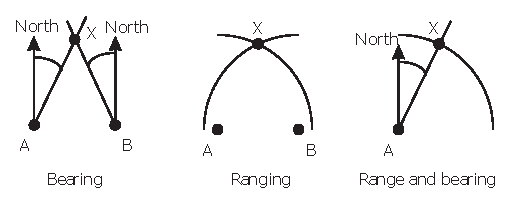
\includegraphics[width=\textwidth]{geometric_methods}    	
	\caption[Geometric positioning methods]{Geometric positioning methods: when the measurements obtained correspond to ranges, range differences or direction angles (bearing), in an ideal error free case, the position could be solved by the intersection of different combinations of the geometric elements defined by those these measurements. Source: Paul D. Groves \cite{groves_principles_2008}.}
	\label{fig:geometric}
\end{figure}
\begin{description}
	\item \textbf{Geometric Methods}
	
	The range, range difference and direction angles values provided by the previously described measurements are not individually enough to know the position of the moving node, as they represent circumferences, hyperboles or lines (spheres, hyperboloids and planes, in the three-dimensional case). 
	However, if several non-redundant measurements are available, a system of equations can be established and the unknown position solved.
	As can seen in the Figure~\ref{fig:geometric} for the two-dimensional case, there are different combinations of the geometrical constraints that can be combined to solve the unknown position: the intersection of three circumferences, of two lines, or a line and a circumference.
	In the three-dimensional case there are a greater number of combinations, being the most common one the intersection of four spheres.
	
	If only one type of geometric constraint is used, specific names are usually used: trilateration for ranges (circumferences or spheres intersections); multilateration for range differences (hyperbolas or hyperboloids intersections); and triangulation for angles (lines or planes intersections).
		
	% Unfortunately, the measurements are not error-free, which generates over-determined systems of equations. 
	% In addition, some of the $\boldsymbol{h}$ functions may be non-linear, so the systems can not commonly be solved analytically. 
	% If the $\boldsymbol{e}$ error is relatively small compared to the $\boldsymbol{z}$ measurements, approximate methods (e.g. least squares), linearized functions and iterative methods can be used.
	
	Unfortunately, since measurements are not usually error-free, the problem becomes an over-determined system of non-linear equations, which cannot commonly be solved analytically.
	If the $\boldsymbol{e}$ error is relatively small compared to the $\boldsymbol{z}$ measurements, iterative methods and approximate closed-form solutions (e.g. least squares) can be applied on linearized functions.
	%%%%%%%%%%%%%%%%%%%%%%%%%%%%%%%%%%%%%%%%%%%%%%%%%%%%%%%%%%%
	\item \textbf{Cost Function Minimization Methods}
	
	%Another approach for the cases where the analytical expression of function $\boldsymbol{h}$ is known and the error $\boldsymbol{e}$ is relatively small is to minimize a cost function such as the following one:
	For cases where the analytical expression of function $\boldsymbol{h}$ is known and the error $\boldsymbol{e}$ is relatively small, one approach is to minimize a cost function such as the following:
	\begin{equation}
	\label{eqn_costFunction}
		V(\boldsymbol{x})=\log p_e(\boldsymbol{z}-\boldsymbol{h}(\boldsymbol{x}))
	\end{equation}	
	where $p_e$ is the probability density function of the error $\boldsymbol{e}$. 	
	This optimization process will maximize the conditional probability $p(\boldsymbol{z}|\boldsymbol{x})$, so maximum likelihood estimators can be obtained for arbitrary error distributions.
	Additionally, it is possible to introduce protections against NLOS situations by converting the optimization problem into a constrained one.
	%%%%%%%%%%%%%%%%%%%%%%%%%%%%%%%%%%%%%%%%%%%%%%%%%%%%%%%%%%%
	\item \textbf{Fingerprinting Methods}
	
	When function $\boldsymbol{h}$ has no analytical expression, or it is difficult to obtain, or if the error $\boldsymbol{e}$ is significant compared to the measurements $\boldsymbol{z}$, methods from the machine learning field are commonly used, often known as fingerprinting.
	
	These methods are based on the previous generation of a map or database and convert the localization problem into a problem of inference or classification.
	Therefore, they consist of two phases: in the first one, known as offline calibration or training, values of the measurements of interest are collected in different positions of the area in which the localization service is to be provided.
	With these measurements, the database is constructed and, subsequently, during the online estimation phase, based on the specific measurements collected by the mobile node, the database is queried and the nearest or most probable position is returned as the estimated one.
	Techniques such as \emph{K-Nearest Neighbors} (KNN), Bayesian decision, \emph{Artificial Neural Networks} (ANN) or \emph{Support Vector Machines} (SVM) are usually applied for the estimation.
	
	These methods are based on relying solely on data collected during the offline phase.
	In this way, they do not need to know more features about the scenario, such as differentiating NLOS and LOS situations, knowing error distributions or even knowing the anchors' positions.
	This allows them to achieve good levels of accuracy.
	%However, their performance depends on the dimensionality of the measurements collected, the granularity with which the training data is done and the environment is not changed.
	However, performance depends on the dimensionality and granularity of the data collected during the offline phase and that the scenario is not modified.
	In addition, that offline calibration phase is often very time-consuming.
\end{description}	
%%%%%%%%%%%%%%%%%%%%%%%%%%%%%%%%%%%%%%%%%%%%%%%%%%%%%%%%%%%%%%%%%%%%%%%%%%%%%%%%%%%%%%%%%%%%
\subsection{Technologies}
\label{sec:2_2_3_technologies}		
The characteristics of signals that can be generated by the technology selected to implement a localization system will determine the type of measurements and estimation methods which are more appropriate, and what performance can be achieved in terms of accuracy, coverage and other requirements.
The following is a brief review of the main technologies used for position fixing based localization systems, focusing on the main strengths, weaknesses and areas of use of each of them.
\begin{description}
	\item \textbf{Global Navigation Satellite Systems}
		
	GNSS is the most widespread type of positioning system, mainly due to its almost global coverage and the availability of receivers integrated in a multitude of devices.
	
	The basis for their operation is the existence of a constellation of satellites whose orbits are known and it is therefore possible to know their position at any given time with good precision.
	The satellites emit electromagnetic signals in the microwave range, which contain modulated pseudo-random codes specifically designed to facilitate the estimation of the ToF between each satellite and receiver.
	Synchronization between the satellites is achieved by means of atomic clocks installed on them.
	On the other hand, the receiver's clock is of poorer quality and contains a certain synchronization error. However, since this error will be common to all satellites that are visible simultaneously, it can be eliminated if at least four satellites are received.
	By obtaining the ranges to at least four satellites, it is possible to compute the three-dimensional position of the receiver by trilateration.	

	The main weaknesses and disadvantages of these systems are:
	\begin{itemize}
		\item The power of the emitted signals is low, making it difficult to receive them with sufficient quality in, for instance, indoor environments or under trees.
		\item The troposphere and the ionosphere affect the propagation velocity of the electromagnetic wave, which results in an error in the estimation of the ranges and, hence, of the position.
		\item The existence of multipaths may also affect the estimation of ranges. This is especially common in NLOS scenarios, such as urban canyons.
		\item The relative geometry between the satellites and the receiver can generate different accuracies in different directions in space. This is usually known as \emph{Dilution of Position} (DoP).
		\item The necessary infrastructure, i.e. satellites, is expensive to produce, install and maintain.
	\end{itemize}	
	In the Table~\ref{table:ch2_GNSS_errors} it can be seen the orders of magnitude of the effect of the different error sources on the position error.
	However, depending on the complexity of the receiver and the amount of corrections applied, it is possible to achieve accuracies of the order of 10 meters for basic receivers to centimeter errors with more advanced solutions such as Differential GNSS or \emph{Real Time Kinematic} (RTK), although its use is mainly limited to outdoors scenarios.	
	\begin{table}[!t]
		%\renewcommand{\arraystretch}{1.3}
		\centering
		%\rowcolors{2}{gray!25}{white}
		\begin{tabular}{c c}
			\hline
			\rowcolor{gray!25}
			\bfseries Source of error & \bfseries Resulting position error\\
			\hline
			Satellites' clock and orbits& 0.5 m – 1 m\\
			\hline
			Atmospheric delays&1 m – 3 m\\
			\hline
			Multipath and NLOS signals&0.1 m – 100 m\\
			\hline
			Receiver thermal noise&0.1 m\\
		\end{tabular}
		\caption[Order of magnitude of the main GNSS position error sources]{Order of magnitude of the main position error sources in GNSS systems. Source:  SaPPART White paper \cite{noauthor_cost_2015}.}	
		\label{table:ch2_GNSS_errors}	
	\end{table}			
	%% Esta figura está bien pero es un poco pequeña %\InsertFig{GNSS.png}{fig:GNSS}{}{}{1}{}	
	%%%%%%%%%%
	\newpage
	\item \textbf{Wireless Local Area Networks}
	
	\emph{Wireless Local Area Networks} (WLAN) is a widely used set of wireless communication protocols (mainly IEEE 802.11) that can also be used for localization. 
	It is precisely this availability of already installed anchors in a multitude of environments and receivers in portable devices such as smartphones or laptops that is its main strength when it comes to being chosen as localization technology.
	%It operates in the ISM (Industrial, Scientific and Medical) bands and its coverage typically ranges 50-100 meters, surpassing other communication technologies.
	
	Propagation delay based measurements are often not used because of the poor results obtained. On the one hand, the off-the-shelf WLAN hardware is not usually ready to measure arrival times and, on the other hand, the usual bandwidth of WLAN systems (typically 20 MHz) implies that any multipath that occurs within 1-2 meters around the receiving node can be indistinguible from the direct path signal. This resolution is not enough for indoor environments with many obstacles in that range.
	
	RSS measurements are usually available on devices, but since WLAN anchors installation is usually designed to optimize communication, not positioning, and its coverage typically ranges 50-100 meters, NLOS situations are common. This makes it difficult to use an analytical propagation model, so fingerprinting-based techniques are the most common.
	
	With these techniques, accuracies between 1 and 10 meters are usually obtained, depending on the number of anchors and the density of calibration points.
	The main disadvantage of using WLAN fingerprinting is the high cost of performing the offline calibration phase, which can be degraded by changes in the environment.
	In addition, RSS values taken by different receiving devices may vary depending on the hardware and the power control strategies performed during data communications, which will also degrade the accuracy of the estimate.
	%%%%%%%%%%
	\item \textbf{Ultra Wideband}
	
	UWB is a communications technology that is defined as having an absolute bandwidth of at least 500 MHz or a relative bandwidth greater than 20\%. 
	It allows short-range communications (less than 100 meters), with high data rate and low power consumption but, thanks to its bandwidth, is especially useful for implementing localization systems based on propagation times. 
	Returning to the equation~\ref{eqn_heisenberg}, a bandwidth of 500 MHz implies a theoretical 5 centimeters range safe against multipaths.
	With these characteristics, position estimation with errors of a few tens of centimeters is achieved.
	However, as this is not a commonly used wireless technology, the systems currently developed are few and more expensive than other adopted technologies such as WLAN.
	
	%%%%%%%%%%
	\item \textbf{Sound}
	
	In contrast to electromagnetic waves, sound is a mechanical wave associated to a pressure oscillation transmitted through a medium, commonly the air.
	In general, signals in the ultrasound range are used, although there are also systems in the audible range to take advantage of the sound cards available in many devices.
	
	The characteristics of these signals involve a number of strengths and weaknesses that result in the use of only propagation delay measurements.
	Regarding their strengths:	
	\begin{itemize}
		\item Since the speed of sound propagation in the air is slow (around 343 m/s at 20°C), it is easy to detect and avoid multipaths, so centimeter-level accuracies can be achieved in indoor scenarios.
		\item This low propagation speed in comparison to the electromagnetic waves also facilitates the synchronization between nodes.
		\item Its hardware components are simple to implement and low cost.		
	\end{itemize}
	As for their weaknesses:
	\begin{itemize}
		\item Its main restriction is the low coverage mainly because of the high attenuation of these waves in the air.
		\item The velocity of sound propagation in the air is highly affected by temperature. This implies the implementation of compensation systems and avoiding environments with large temperature changes, such as outdoors.
		%\item In addition to NLOS and multipath situations, it is also sensitive to the Doppler effect if the nodes are moving at considerable speeds.		
		\item In addition to NLOS and multipath situations, due to the low propagation speed, these systems are also sensitive to the Doppler effect if the nodes are moving at considerable speeds.
	\end{itemize}
		
	%These characteristics mean that sounds are rarely used outdoors, often limited to confined spaces with few NLOS situations, and for applications requiring high levels of accuracy. 
	These characteristics make sound waves rarely be used outdoors, limiting their use to small spaces, avoiding NLOS situations and especially for applications that require great accuracy.
	In addition, the availability of high accuracy implies that the positions of the anchors must be known with at least the same accuracy, which complicates the installation process.
	%%%%%%%%%
	\item \textbf{Bluetooth Low Energy}	
	
	\emph{Bluetooth Low Energy} (BLE) is a wireless communication technology that offers simple devices the ability to exchange small amounts of data with very low power consumption.
	One of the most common operating modes is advertising, which allows a node to broadcast short messages periodically.
	These messages and their RSS measurements can be used to detect the proximity to one of these beacons and to estimate the position of a mobile node.
	
	The main advantages of this technology are the availability of receivers in many electronic devices, their high security, low cost and low consumption.
	The standard allows coverage ranges up to 100 meters but most beacons are usually visible from no more than 10 meters.
	
	This low coverage means that the main estimation technique is proximity and symbolic localization, which may be sufficient for some applications such as shopping centres or museums.
	However, it is also possible to apply fingerprinting techniques that give similar results to those achieved with WLAN and even to use analytical propagation models, which can achieve good results if the mobile node is about one meter away from the transmitter.
	
	In addition to the low coverage, another of its main disadvantages is that the low frequency of advertising can generate a latency in the estimation of the location, which makes real time applications difficult.	
\end{description}
% \InsertFig{tecnologies_comparison_Mautz.png}{fig:Mautz}{Comparison of accuracy and coverage offered by different technologies for position fixing localization method.}{Source: Rainer Mautz \cite{mautz_rainer_indoor_2012}}{1}{}
\begin{figure}[!t]
    \centering
	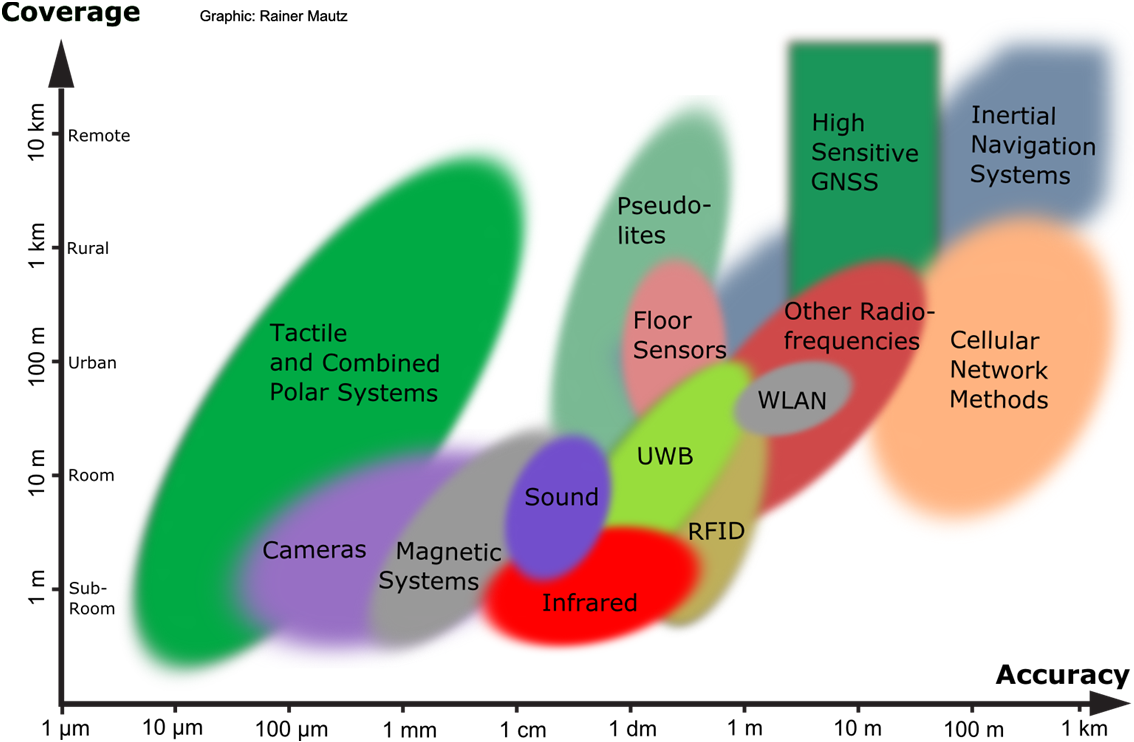
\includegraphics[width=\textwidth]{tecnologies_comparison_Mautz}    	
	\caption[Comparison of position accuracy and coverage offered by different technologies]{Comparison of accuracy and coverage offered by different technologies for position fixing localization method. Source: Rainer Mautz \cite{mautz_rainer_indoor_2012}.}
	\label{fig:Mautz}
\end{figure}

There are many other technologies that can be used to implement localization systems based on position fixing: cameras, infrared, RFID, visible light, magnetic fields, cellular networks and even television and FM radio signals. 
%The difference in the choice of technology is mainly reflected in the balance between accuracy and coverage, which is shown visually in the Figure~\ref{fig:Mautz}.
%When choosing a technology, one of the first features to consider is their balance between accuracy and coverage provided by the basic installation (obviously, it can always be scaled up to cover bigger areas).
When choosing a technology, one of the first features to consider is their balance between accuracy and coverage.
In Figure~\ref{fig:Mautz} can be seen a comparison of the most common technologies.
%In Figure~\ref{fig:Mautz} can be seen a comparison of this feature for the most common technologies, obviously considering only the installation of the basic infrastructure needed for each of them, since any solution can be scaled up to global coverage.
In addition to this compromise between accuracy and coverage, the main characteristic that summarizes the performance of the position fixing localization methods is that they offer better accuracy in the long-term than in the short-term. 
That is, there may be times when, because of NLOS or multipath situations, or temporary interferences, the position estimation error increases but, on average, it tends to be bounded.